\documentclass{article}

\usepackage[utf8]{inputenc}
\usepackage{graphicx} % For including images
\usepackage{listings} % For code snippets
\usepackage{amsmath} % For mathematical equations
\usepackage{hyperref} % For hyperlinks
\usepackage{tikz}

\title{Robot Arm GUI Controller Via Network}
\author{Eduards Abisevs}
\date{\today}

\begin{document}

\maketitle
\tableofcontents
\newpage

\section{Introduction}

\section{Project Goals and Objectives}

\section{Theory}
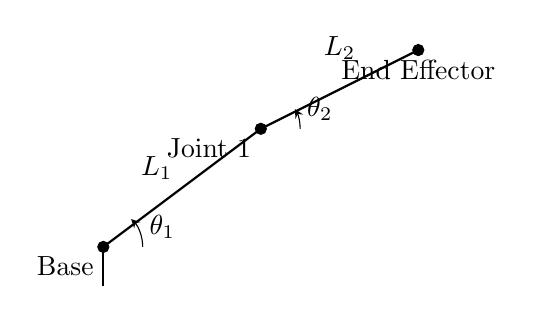
\begin{tikzpicture}

% Base
\draw[thick] (0,0) -- (0,0.5);

% First Link
\draw[thick] (0,0.5) -- (2,2);
\node at (1,1.5) [left] {$L_1$};

% Second Link
\draw[thick] (2,2) -- (4,3);
\node at (3,2.75) [above] {$L_2$};

% Joints
\filldraw[black] (0,0.5) circle (2pt) node[anchor=north east] {Base};
\filldraw[black] (2,2) circle (2pt) node[anchor=north east] {Joint 1};
\filldraw[black] (4,3) circle (2pt) node[align=center, below] {End Effector};

% Angle Annotations
\draw[->,>=stealth] (0.5,0.5) arc (0:45:0.5);
\node at (0.75,0.75) {$\theta_1$};

\draw[->,>=stealth] (2.5,2) arc (0:30:0.5);
\node at (2.75,2.25) {$\theta_2$};

\end{tikzpicture}


\end{document}

